\section{Beskrivelse av virksomheten}

% Aktuelle avdelinger, seksjon, stilling, funksjon, osv.
\subsection{Avdelinger, seksjon, stilling, og funksjon}
Solwr Software er en del av Solwr-virksomheten, som også inkluderer Solwr Robotics. Disse to underavdelingene fokuserer på programvareutvikling og robotikk, med ulike prosjekter og avdelinger. Innen Solwr Software er det tre avdelinger med et prosjekt hver for praktikantene: matematikk-rettet, backend-rettet, og frontend-rettet. Praksisarbeidet mitt var knyttet til det matematiske-rettede prosjektet, som er prosjektet til \gls{rnd} avdelingen. \Gls{rnd} er ansvarlig for prosjektet jeg jobbet på. Der ble det gjennomført et forprosjekt med hensikt på å utvikle en prototype for en \gls{abc} analyse-modul som i fremtiden skal integreres i selskapets hovedapplikasjon.

\subsection{Ytre forhold}
Kontorlokalene til virksomheten er moderne og godt tilrettelagt for både individuelle arbeidsoppgaver og samarbeid i team. Fasilitetene inkluderer:

\begin{itemize}
    \item Kontorplasser: Utstyrt med laptoper, aller har minst én skjerm, og tavler fra gulv til tak for å skrive ned og notere.
    \item Fellesområder: En kantine med salatbar, varm drikke maskin, og sittegrupper som øker sosial stimuli, som blant annet en sjakkkrok.
    \item Møterom: hovedkontoret har flere møterom for gruppearbeid og ideutvikling.
\end{itemize}

Mitt arbeidsområde var i kontoret til \gls{rnd}, hvor jeg hadde egen sitteplass ved siden av veilederen.

\begin{figure}[H]
    \centering
    \subfloat[\centering Alle sitteplassene i \gls{rnd} sitt kontor.]{{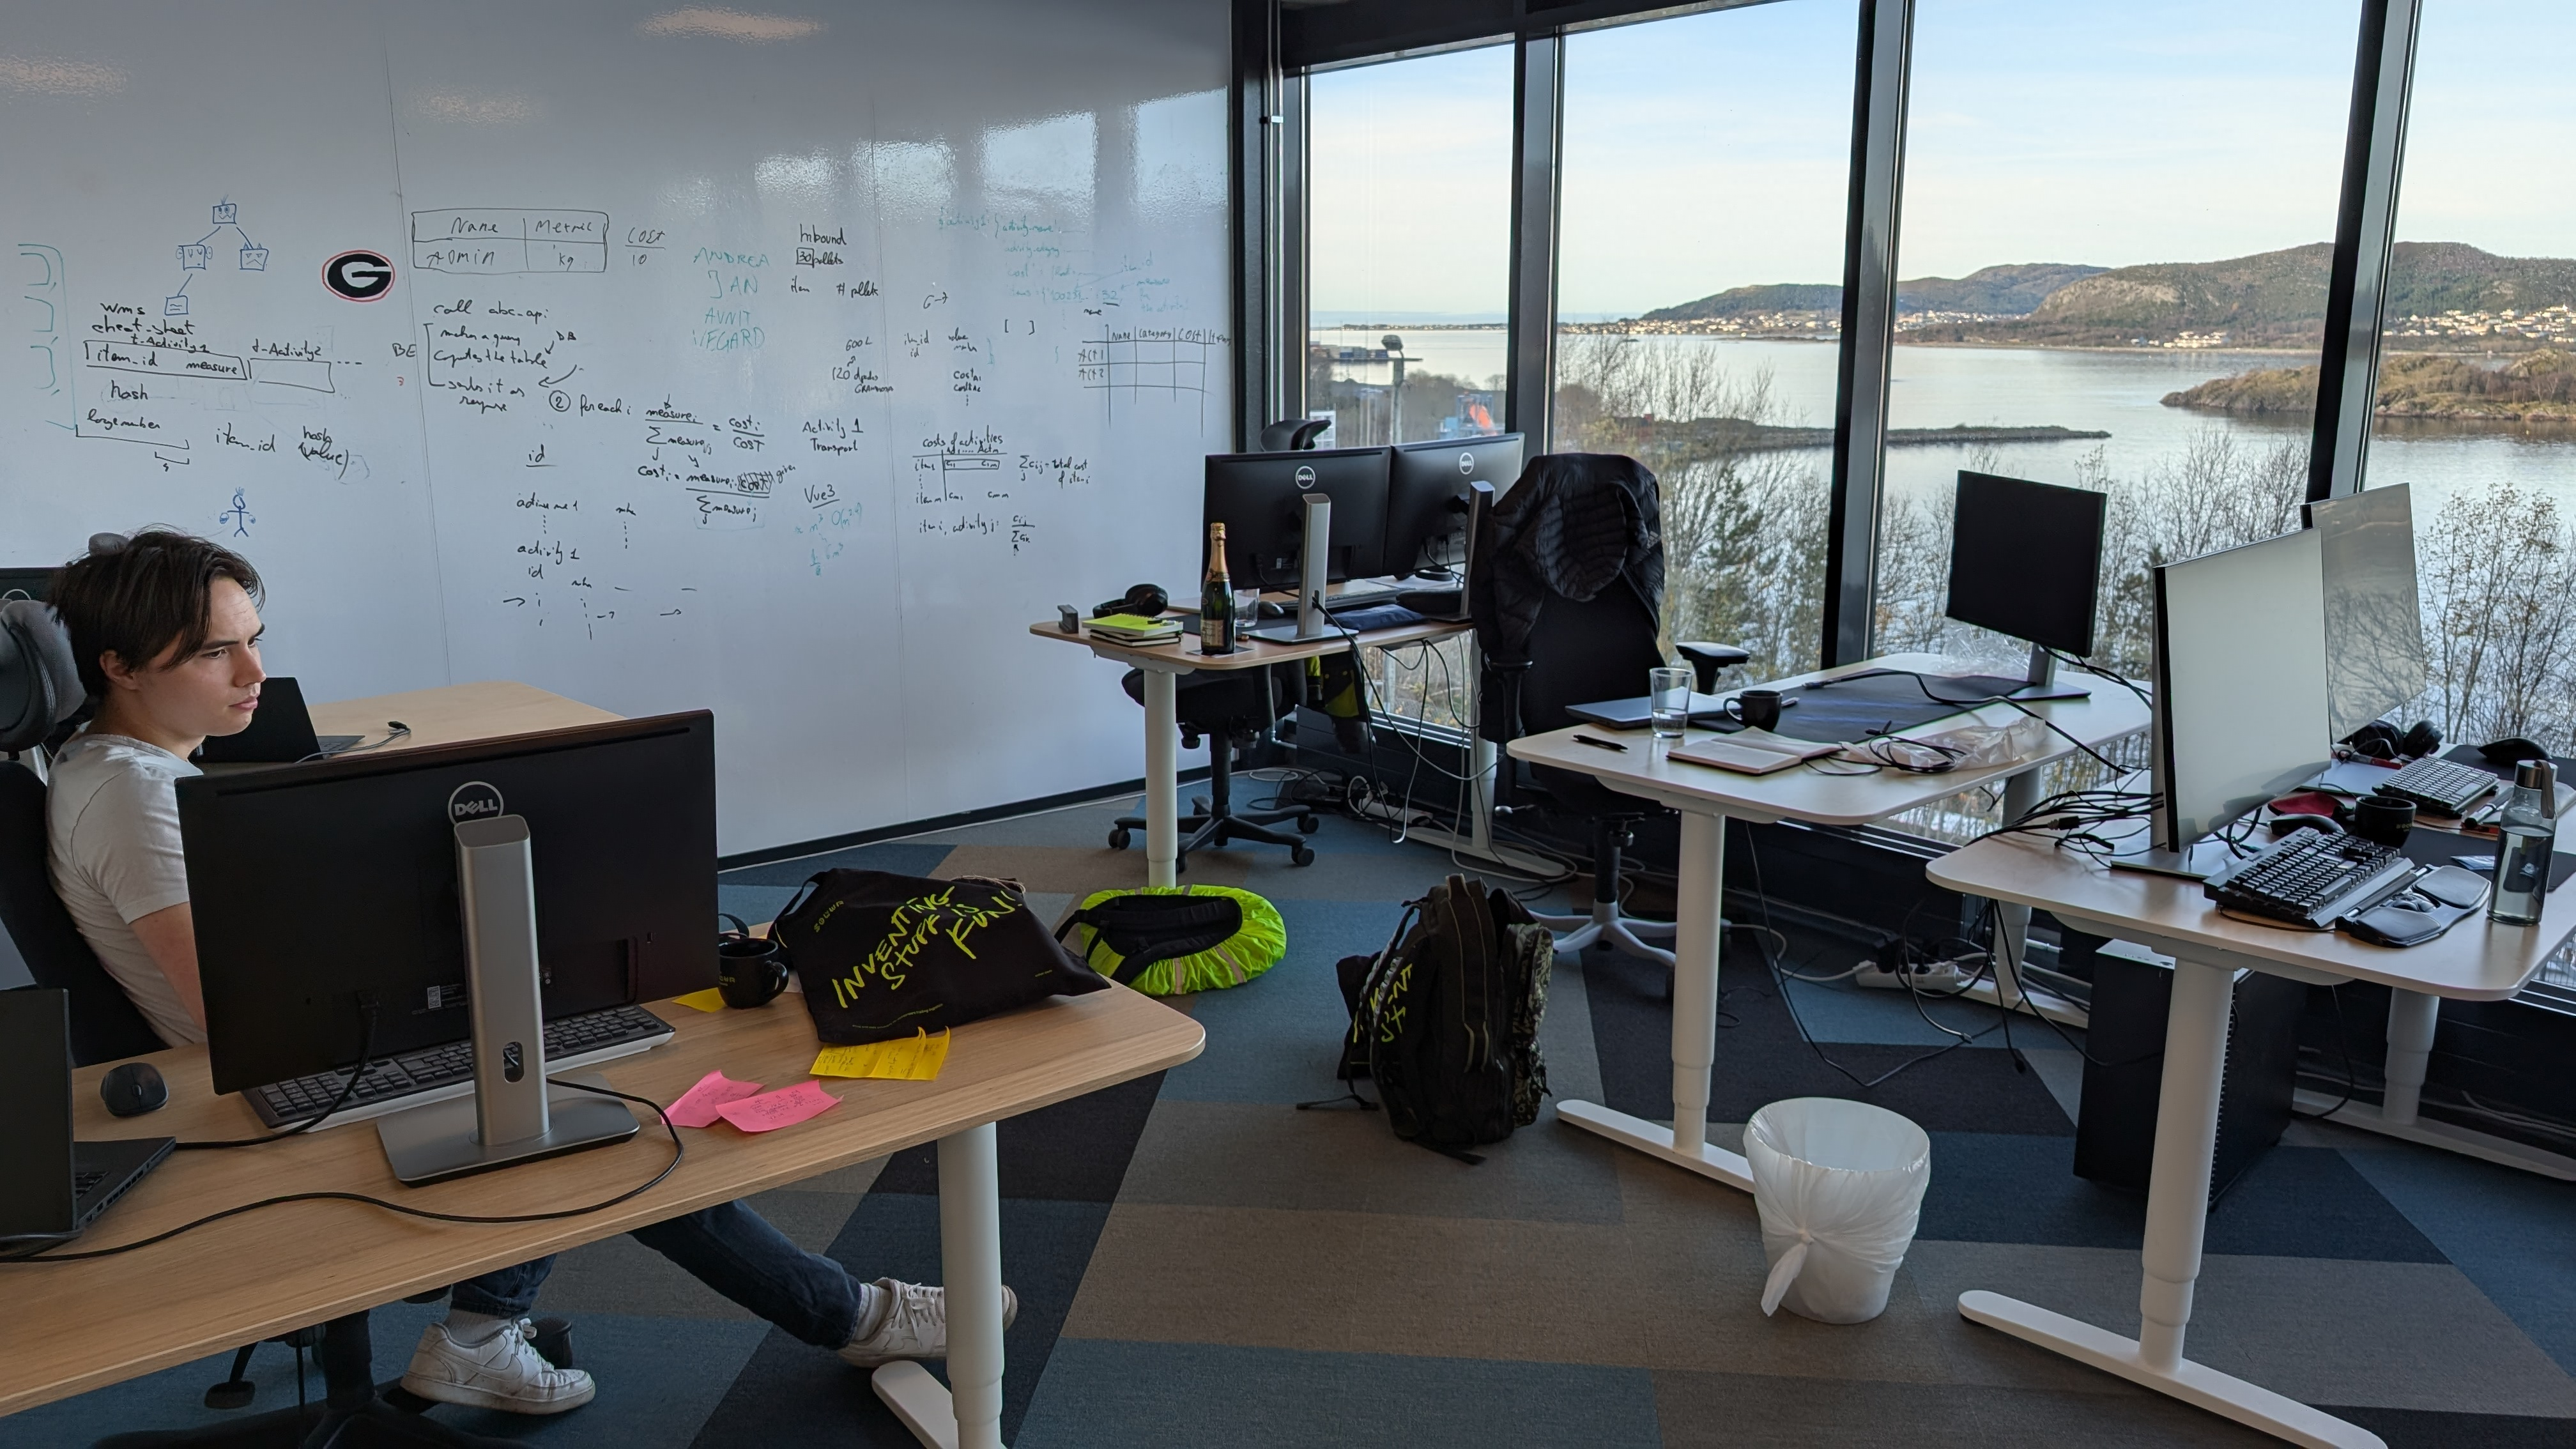
\includegraphics[width=0.45\linewidth]{resources/location/rnd_office.jpg}}}
    \qquad
    \subfloat[\centering Studenten sin sitteplass under praksisen.]{{\includegraphics[height=0.45\linewidth]{resources/location/where_i_sat.jpg}}}
    \caption{\label{fig:kontoret_til_rnd}Kontoret til avdelingen.}
\end{figure}
 
% Prosesser og oppgaver i virksomheten som er særlig relevante i forhold til praksisen beskrives.
\subsection{Prosesser og oppgaver}
% \color{red}
% Det ble holdt statusmøter mellom veileder og \gls{rnd} praktikantene. I disse møtene ble det diskutert \dots
% \color{black}
% \color{red}
Solwr har tydelig strukturerte prosesser for å utvikle og teste løsninger som oppfyller kundenes behov. I praksisperioden var spesielt følgende prosesser og oppgaver relevante:
\begin{itemize}
    \item \textbf{Utvikling av \gls{trace}:} \gls{trace} er en sentral plattform som brukes til å samle, visualisere og bearbeide data fra ulike systemkomponenter. I praksisperioden min deltok jeg i å bygge på nye funksjoner.
    \item \textbf{\gls{abc}-modulen:} Praksisen sitt hovedfokus var å integrere denne modulen inn i \gls{trace}. Dette var et forprosjekt for å utvikle en prototype for å utføre \gls{abc}-analyser. Dette involverte:
    \begin{itemize}
        \item Skrive komplekse \gls{sql}-queryer for å hente og bearbeide data.
        \item Utvikle en \gls{api} for backend-funksjonalitet.
        \item Lage frontend-komponenter for visualisering av data og internasjonalisering.
    \end{itemize}
    \item \textbf{Iterativ utviklingsprosess:} Arbeidet ble gjort steg for steg, der jeg jobbet sammen med veileder og andre praktikanter. Vi brukte verktøy som \gls{git} for versjonskontroll og Postman for testing, og hadde statusmøter for å sikre fremdrift.
    \item \textbf{Teamarbeid:} Selv om veilederen min var hovedkontakten, samarbeidet jeg også med andre ansatte i \gls{rnd}-teamet. Dette ga meg erfaring med å jobbe i et tverrfaglig miljø, noe som var både inspirerende og lærerikt.
\end{itemize}
Gjennom disse oppgavene fikk jeg en god blanding av praktisk erfaring og teoretiske utfordringer, og jeg lærte mye om hvordan teknologi brukes i hverdagen på arbeidsplassen.
% \color{black}

\subsection{Relevans for praksisen}
Solwrs fokus på innovasjon og utvikling gjorde virksomheten til en ideell arena for praksisopplæring. Bedriften la til rette for praktisk læring i et realistisk arbeidsmiljø, hvor både tekniske ferdigheter og evnen til samarbeid ble satt på prøve. Prosjektet jeg jobbet på, hadde en direkte kobling til fagområdene innen programvareutvikling og anvendt matematikk, noe som bidro til en verdifull praksisopplevelse.